\chapter{相关工作与前置知识}

\section{被动感知技术的应用}
被动感知技术的应用广泛,这里我们主要介绍本课题涉及到的两个方向:环境感知和人机交互。
\subsection{环境感知}
环境感知是智能感知领域的一个研究方向\upcite{vukovic2004adaptive}。赋予终端环境感知的能力,可以使之更加了解用户所处的环境状态,提供更加智能化的服务。普遍意义上的环境包含物理环境,用户环境,计算环境三个方面。一,计算环境,主要包含网络连接、通信带宽、临近资源等信息;二,用户环境,主要包含状态、位置、社交情况等信息;三,物理环境,包含光线、噪音,温度、湿度和交通流量等信息。

本文主要研究物理环境的感知。研究人员发明的各种各样的传感器可以帮助设备感知声音、光线、温度、湿度等基本物理环境因素,但基于基本物理因素的上层综合物理环境的感知研究依然有很多问题悬而未决。例如对用户危险状态的感知,对用户周围交通流量的感知,对用户周围人员密度的感知,对用户人体动作的感知,这些都是可深入研究的领域。

\subsection{人机交互}

科技在高速发展,需求不断增多,人机交互技术也在不断更新:从机器的被动接受指令到主动获取输入,从人类单向输入到人机的双向交流,从有线的连接到无线的交互。“科技改变生活”这句话在人机交互领域有直观的体现。

\subsubsection{被动接受与单向输入}

18世纪初,意大利人Alan Mathison Turing发明机械打字机,但当时并没有流行起来。随后美国对一位叫William Gilber的人发明了排字机,重定义了打字机,并取得了相应专利。排字机可以说是现代键盘原型。基于排字机,美国的Christopher Latham Sholes于18世纪60年代发明了QWERTY键位的键盘,沿用至今。

随着人们对计算机的使用场景增多,单纯的键盘已经无法满足人们和计算机交互的需求,接着,鼠标便被发明。19世纪60年代,美国人Douglas Carl Engelbart发明了鼠标,让人们感受了到与计算机交互的顺畅体验。通过鼠标,人们可以自由地点击屏幕上的任何位置,大大提高了使用计算机的体验和处理数据的效率。

但此时的人机交互过程,计算机依然是一个被动角色,只会被动等待输入用户输入指令。
\subsubsection{主动获取与双向交流}

低效笨拙的被动等待输入式交流方式很快便无法满足人们的需求。直到苹果推出以Siri为代表的智能语音助手,它们不仅交互简单,而且会主动搜索,推测用户真实意图。

Google公司紧接着也推出了自己的语音助手Google Now,Google Now 的服务依托于Google强大的搜索功能,它记录用户搜索关键字,预判用户意图,并主动向用户提供建议和服务。这让设备从被动回答用户的提问升级为主动获取用户输入并推测用户意图,并主动为人类提供服务的交互方式。

进一步,当微软推出了Kinnect体感交互系统,人与计算机的交互也来到了一个全新的阶段。这一阶段,设备已经变被动为主动,已经开始主动获取输入。

\subsubsection{人机交互技术趋势}

一方面,从机器到角度讲,其与人的交互方式是从被动输入到主动获取。另一方面,从人的角度讲,其与机器的交互设备从有线的键盘鼠标到无线的远程遥控,再到无设备的体感交互。不难看出人机交互技术的趋势是从机器被动到机器主动,从有线到无线,从特制专用设备到普适感知。

\subsection{被动感知的优势}
被动感知的优势是其不需要目标的配合,因而具有很强的普适性。在计算机领域普适性和易部署是系统设计时必须要考虑的一个问题。比如,计算机领域最传统的网络安全性问题,虽然研究人员已经设计了各种办法解决这个问题,但由于这些需求普遍需要升级全网的设备,不具有普适性和易部署性,导致现在网络攻击依然是一个很棘手的问题。而被动感知由于不需要目标的配合,不存在于目标端部署的问题。

被动感知大多基于无线的方式实现,可以摆脱线缆的限制。如今电子设备随处可见,与设备有关的线缆似乎更是随处可见。作者本人更是对线缆十分厌恶,线缆不仅不方便携带,还十分不美观。无线网络,无线充电,无线耳机,各种新技术都预示着未来是无线的天下。基于智能终端的感知必然也要选用无线的技术。试想一个小小的智能终端,接上一堆比自身体积还要大的线缆,那简直是噩梦般的体验。

此外,基于被动感知的终端具有隐蔽的特性,不易被检测,在安防方向有很大的应用前景。


\section{相关工作}
%基于可见光,RSSI,FM,CSI

\subsection{基于摄像头的环境感知技术}

%手势识别,基于摄像头的汽车靠近检测,安防(环境感知)

摄像头作为电子设备上功能最类似人眼的部件,其应用场景的想象空间巨大。理论上来人类通过眼睛可以获取到的信息,智能终端也通过摄像头获取到。在过去的几十年里,机器视觉领域的研究发展迅速,各种技术已趋于产品化。产品方面有基于摄像头的人类识别,车牌识别,运动物体追踪等等。在学术研究上有基于摄像头检测司机是否安全驾驶汽车,帮助行人观察是否有危险车辆靠近,识别用户的手势动作等。

日本三菱电子公司的研究人员就基于摄像头实现了一个可以实时检测、跟踪和识别交通标志的车载系统\upcite{mogelmose2012vision}。作者提出了一种基于均值漂移的通用检测框架。相对于传统模式识别方法,该框架有效提高了识别正确率,减少了误报率。 

达特茅斯大学的Tianyu Wang\upcite{wang2012walksafe}提出了一种基于摄像头检测危险车辆靠近的办法。考虑到行人边打电话边衡穿马路容易引起交通事故,作者据此设计了利用手机摄像头帮助用户感知汽车的系统WalkSafe。WalkSafe主要基于图像识别算法实现。由于图像的处理是一个高计算量的工作,单一智能手机无法胜任,于是作者又设计了离线训练-在线检测的框架,如图~\ref{fig:relatedworkcamera}所示。经实验验证,该方法识别成功率可达80\%左右。
\begin{figure}[htbp] % use float package if you want it here
  \centering
  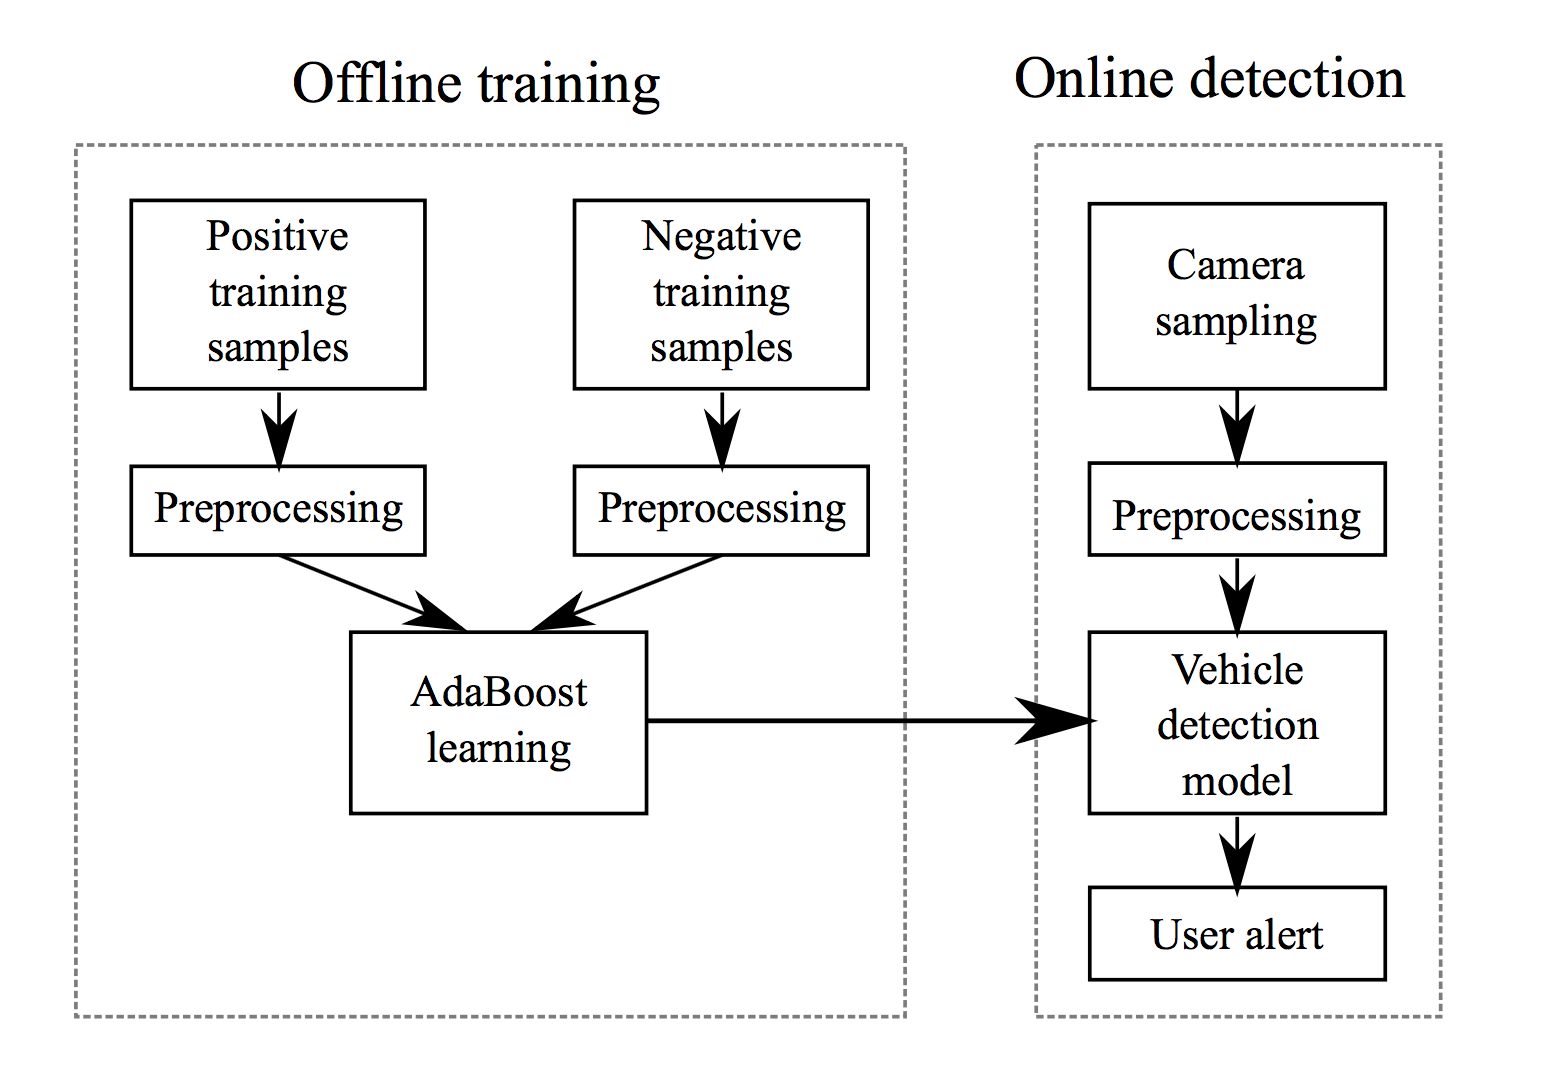
\includegraphics[width=3in]{relatedworkcamera}
  \caption[基于摄像头的危险车辆检测框架]{基于摄像头的危险车辆检测框架(来自文献\upcite{wang2012walksafe})}
  \label{fig:relatedworkcamera}
\end{figure}

基于摄像头的人体动作、手势识别在市面上也已经出现了成熟的产品。比较典型的代表有手势识别产品Leap motion和微软的体感交互产品Kinect。其中Leap motion已经成功应用在了平板等电子设备上,识别精度也可达到手指级别,如图~\ref{fig:leapmotion}。Kinect在游戏领域也得到了广泛的应用,越来越多的针对Kinect设计的游戏发行出来。

\begin{figure}[htbp] % use float package if you want it here
  \centering
  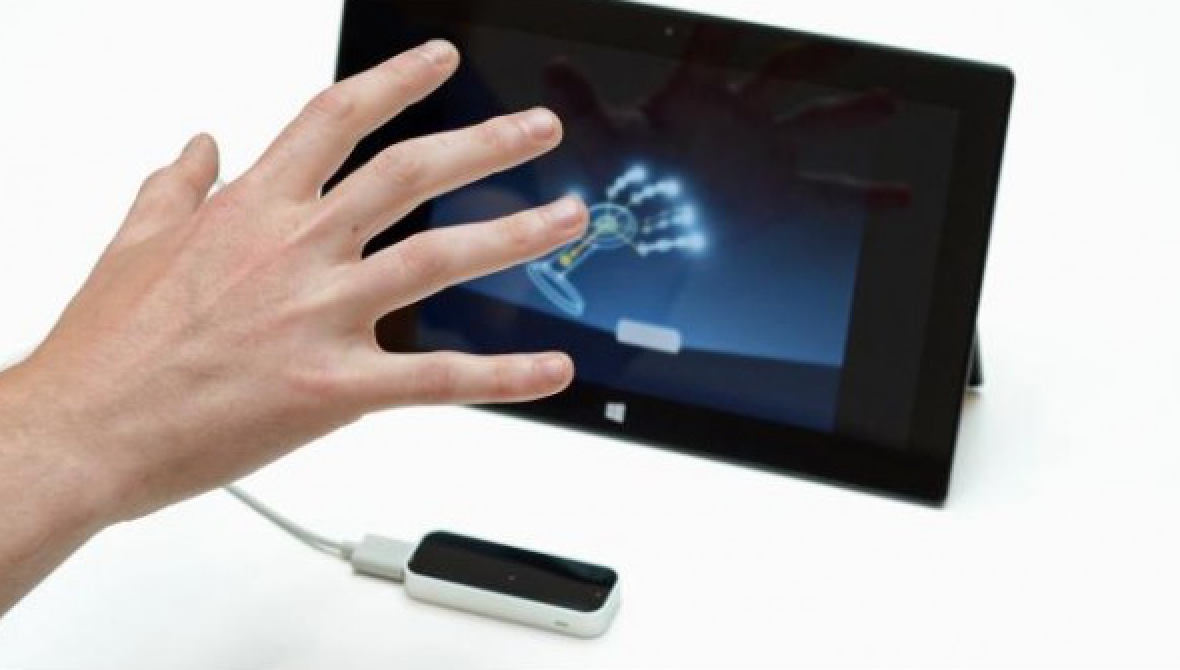
\includegraphics[width=3in]{leapmotion}
  \caption{Leap motion的手势识别产品}
  \label{fig:leapmotion}
\end{figure}


\subsection{基于麦克风的声音感知技术}
声音作为一个类似人耳的传感器,其感知能力不可小觑。随着智能手机终端硬件配置的提升,将声音处理的复杂技术应用到智能终端上称为可能。

贝尔实验室的Nicholas\upcite{lane2015deepear}等人,成功将针对语音的深度学习移植到了移动设备。他们基于深度神经网络开发了一款语音处理框架DeepEar,模型中用到的参数数量达到了$2.3 M$,极大的提升了系统对环境的鲁棒性。该框架经受了多达168个不同环境下的性能评估,表现令人满意。识别正确率高,且耗电小。一天只会消耗移动设备6\%的电量。

声音可以用来感知手势,这是一项很酷的应用。普通人不可能通过耳朵来分别不同手势之间的差异,机器却可以。麦克风所能接收的声音频段远宽于普通人耳能听到的频段,从此角度看,麦克风对声音的感知能力是超过人耳的。基于这一理念,微软亚洲研究院、华盛顿大学合作研发了基于声音的手势识别技术\upcite{gupta2012soundwave}。如图~\ref{fig:soundwave}所示,研究员先利用设备自带的扬声器连续播放固定频率的高频声音,再通过设备的麦克风接收声音。根据多普勒效应,当用户在声音的传播路径上挥手时,麦克风接收到的声音的频率就会发生变化。研究员通过捕捉这种变化来判断用户挥手的方向,从而实现了手势控制浏览器前进后退的功能。
\begin{figure}[htbp] % use float package if you want it here
  \centering
  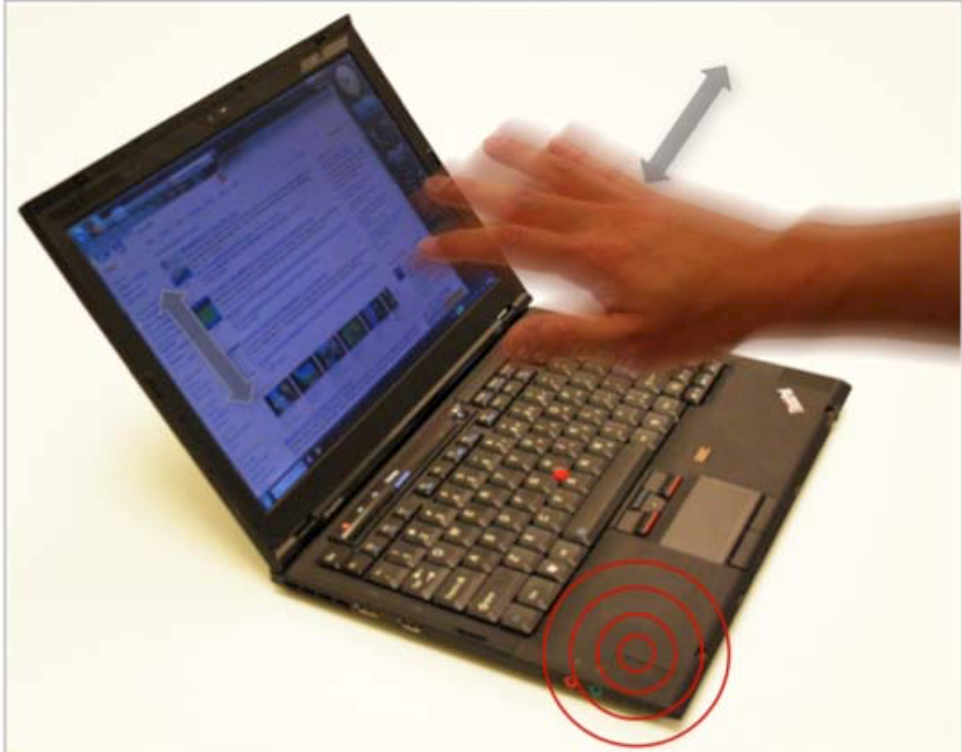
\includegraphics[width=3in]{soundwave}
  \caption{基于声波的手势识别产品}
  \label{fig:soundwave}
\end{figure}

\subsection{基于无线信号的位置感知与追踪技术}
利用无线信号进行位置感知的优势是其抗干扰性。因为如今无线信号就像空气一样,虽然看不到,但是它已遍布我们生活中的任何角落。生活中常见的无线信号有:FM广播,手机通讯信号,Wi-Fi,蓝牙,NFC等。这些信号都曾被用来做位置感知的研究。基于手机信号的室外位置感知目前已十分成熟,精度基本可以满足人们对室外定位的需求。因此近些年研究的热点主要集中在室内定位\upcite{chen2015fusion,zhang2013senstrack}和轨迹追踪\upcite{renaudin2014magnetic,chen2012fm,wu2013will}方面。

Yin Chen\upcite{chen2012fm}等研究员就研究了基于FM信号强度和Wi-Fi信号强度的室内位置感知。相比于基于Wi-Fi信号的室内定位,FM的优势在于其频率低,波长长,受环境中人的影响小。Wi-Fi信号强度会随着时间改变,而FM信号强度受时间的影响要明显小于Wi-Fi信号。除此之外,FM还有传输距离长,功耗小等优点。而Wi-Fi虽然波长短,易受多径效应等影响,但其识别精度高。因此Yin Chen等研究员通过融合两种信号指纹库,来提高室内定位在房间级和米级的精度,如图~\ref{fig:fm}所示。作者分别在商场,公寓,办公室三种室内空间做了测试,均达到了不错的效果。

\begin{figure}[htbp] % use float package if you want it here
  \centering
  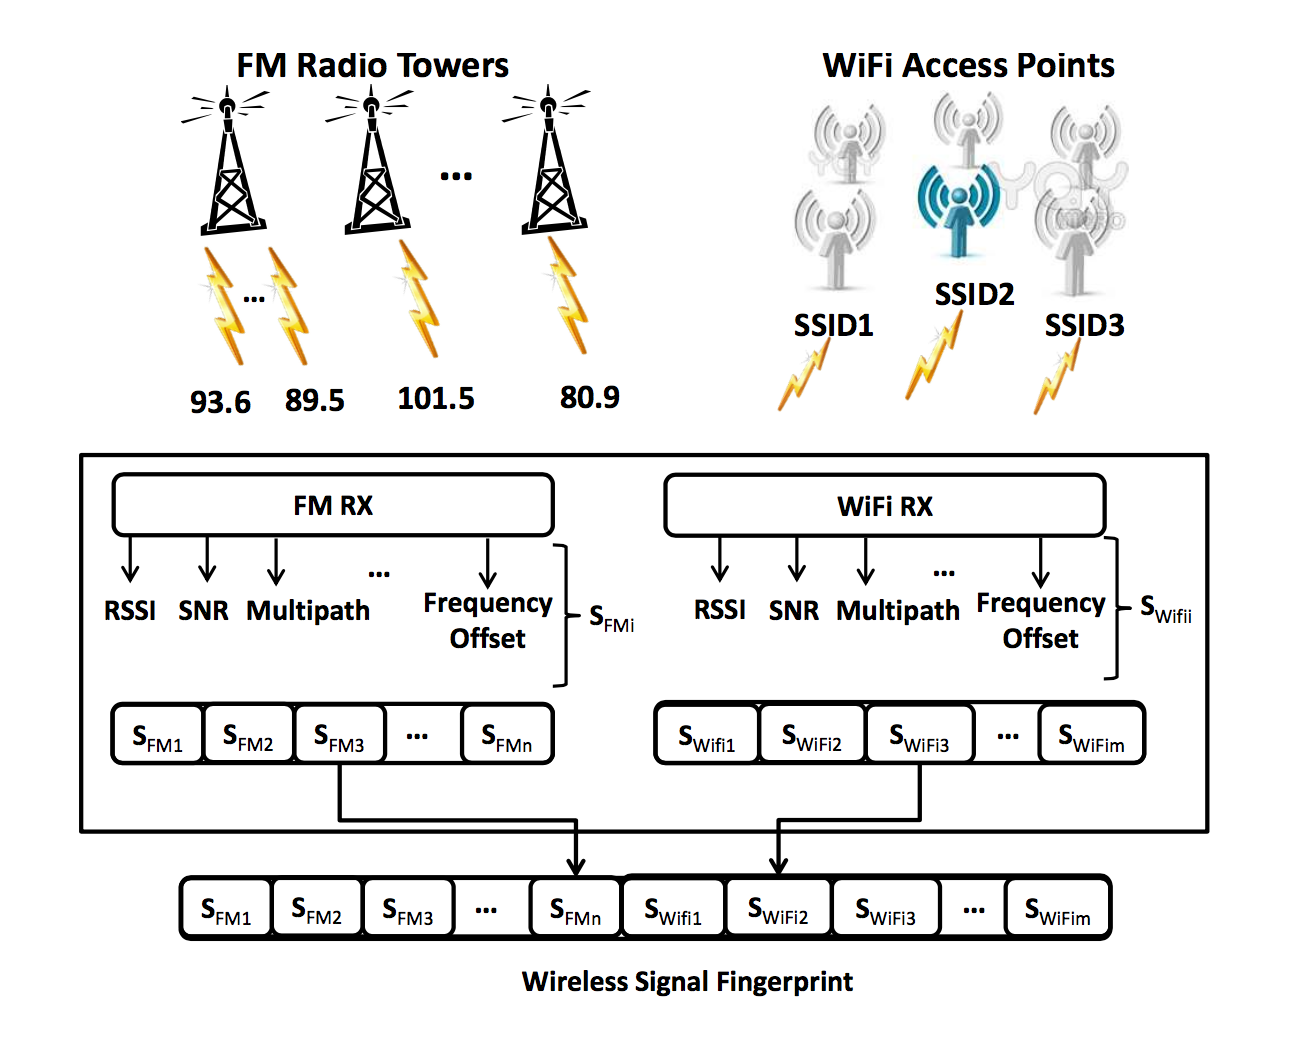
\includegraphics[width=3in]{fm}
  \caption[用FM和Wi-Fi指纹库室内定位]{用FM和Wi-Fi指纹库室内定位(来自文献\upcite{chen2012fm})}
  \label{fig:fm}
\end{figure}

%Wi-Fi 键盘

\subsection{基于无线信号行为识别技术}
无线信号不仅可以用来做定位,还可以用来识别人的具体行为。

清华大学的Xiaolong\upcite{zheng2016smokey}等人研究了基于Wi-Fi感知人们在公共场所吸烟行为的方法。公共场所禁烟是北京这几年的一项新举措,然而实施起来却存在相当大的难度。通过技术手段来实现自动检测吸烟人员是一种不错的思路。该项技术必须要满足两个特点:一是被测者不需要携带任何设备,二是检测设备要布置的很隐蔽。因此基于Wi-Fi信号的检测成了最好的选择,一方面大型公共场所都架设有Wi-Fi,此方法不需要额外增加设备。另一方面,Wi-Fi信号可以穿墙,完全可以布置到隐蔽的地点。另外,此种方法不需要在被检测目标身上部署任何设备,符合实际应用场景。Xiaolong等人把吸烟的行为分解成握烟,抬手,吸烟,放手,吸气,呼气几个子动作,然后分别检测子动作,根据上下文环境推测是否有人在吸烟,其框架~\ref{fig:smokedetection}如图所示。

\begin{figure}[htbp] % use float package if you want it here
  \centering
  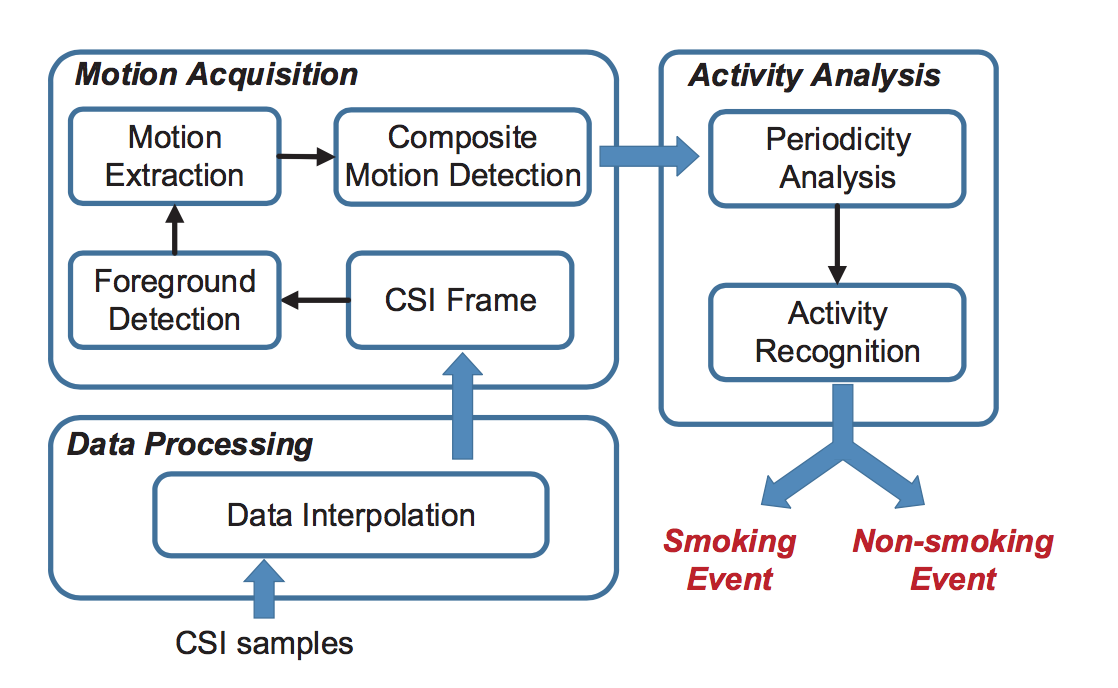
\includegraphics[width=3in]{smokedetection}
  \caption[利用通用Wi-Fi设备检测吸烟行为系统框架]{利用通用Wi-Fi设备检测吸烟行为系统框架(来自文献\upcite{zheng2016smokey})}
  \label{fig:smokedetection}
\end{figure}

Wi-Fi信号还可以用来感知人的行走方向\upcite{wu2016widir}。在典型的智能家居等应用场景中,人的行走方向是一个非常重要的上下文信息。文献\cite{wu2016widir}中就详细介绍了基于Wi-Fi信号CSI数据判断用户行走方向的技术WiDir。人的走动会影响Wi-Fi信号接收端的信道状态信息。作者基于菲涅耳带模型对子载波CSI的相位进行了分析,成功推测出了用户的行走方向。除此之外,作者还基于商用Wi-Fi设备设计实现了一个可以检测用户行走方向的原型系统。评估结果显示该系统的平均检测错误率在10\%以下。

更近一步的,Wi-Fi信号还可以用来进行步态识别,即根据一个人走路的状态确定一个人的身份。这项研究由南京大学的Wei Wang\upcite{wang2016gait}进行。Wei Wang基于商用Wi-Fi设备开发了可以识别用户细粒度的步态特征,从而判断用户身份的步态识别系统WifiU。其应用场景如图~\ref{fig:wifiu}所示。基本思想是,每个人的走路的方式都不完全相同,其对Wi-Fi信号的CSI造成的影响也不同,通过提取CSI中的特征,与用户特征库比对,便可以判断用户的身份。经过作者的评估,此种方法最高可达93.05\%的准确率。
\begin{figure}[htbp] % use float package if you want it here
  \centering
  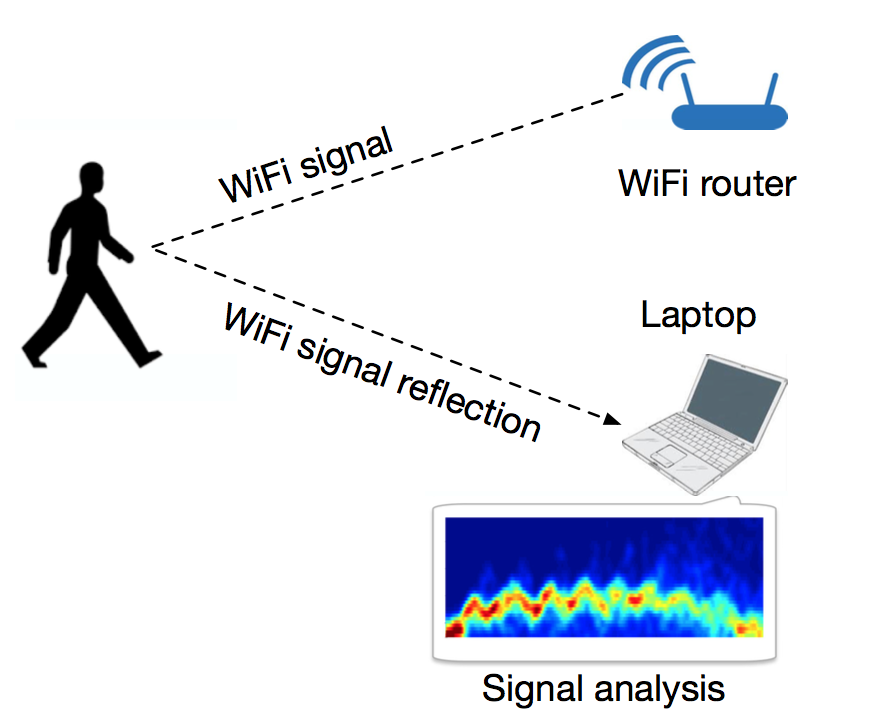
\includegraphics[width=3in]{wifiu}
  \caption[利用Wi-Fi进行步态识别的应用场景]{利用Wi-Fi进行步态识别的应用场景(来自文献\upcite{wang2016gait})}
  \label{fig:wifiu}
\end{figure}



\section{前置知识}

\subsection{音频分析方法}
\subsubsection{快速傅里叶变换}
音频频域信息是由时域信号分解转换后得到的,这一分解过程被称为傅里叶变换(Fourier Transform, FT)。对于时域上离散的音频信号,采用离散傅里叶变换进行分解(Discrete Fourier Transform,DFT)。假设一段有限的离散信号$x(m)$,其长度为$N$,则DFT公式如~\ref{equ:chap3:dft}所示。

\begin{equation}
\label{equ:chap3:dft}
X\left( k \right) = \sum\limits_{m = 0}^{N - 1} {x\left( m \right){e^{ - j{\textstyle{{2\pi } \over N}}mk}},k = 0,...,N - 1}
\end{equation}

公式~\ref{equ:chap3:dft}中有两个整型变量:$m$和$k$。其计算复杂性为$O\left( n^2 \right)$,为了减小计算复杂性,快速傅里叶变换(Fast Fourier Transforms, FFT)应运而生。本文中使用的FFT版本为MIT研究员实现的FFTW\upcite{frigo1998fftw}。


\subsubsection{小波分析}
小波分析\upcite{torrence1998practical}是指用有限长或者快速衰减的振荡波形,即母小波来表示信号。母小波通过平移和缩放等方式匹配原始输入信号。
小波的概念由Grossman和Morlet提出。他们用法语ondelette来表示小波。英语中,被改成了wavelet。
小波变换分为两类,即离散小波变换和连续小波变换。连续变换于所有平移和缩放的全集上变换,离散变换只于所有平移和缩放的某个子集上变换。

小波变换可视为原始信号的时频域表示。表面上类似短时傅里叶变换,但小波变换具有在高频的时间分辨率高,在低频时间分辨率低的特性,正符合我们对信号分析时对分辨率的要求。低频时,例如,频率从1Hz变到2Hz,频率相差一倍,此时频率变化相较时间变化是比较明显且重要的,然而高频时,例如频率从1000Hz变到1001Hz,频率相较时间的变化并不大,对时间分辨率的要求不高。而短时傅里叶变换的分辨率并不会随频率变化,图~\ref{fig:STFT_and_WT}显示了两者分辨率变化的不同。

\begin{figure}[htbp] % use float package if you want it here
  \centering
  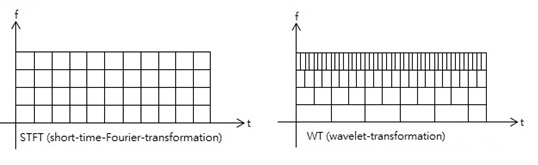
\includegraphics[width=5in]{STFT_and_WT}
  \caption{短时傅里叶变换和小波分析分辨率变化比较}
  \label{fig:STFT_and_WT}
\end{figure}


一个典型的母小波波形如图~\ref{fig:Wavelet-Meyer}所示。
\begin{figure}[htbp] % use float package if you want it here
  \centering
  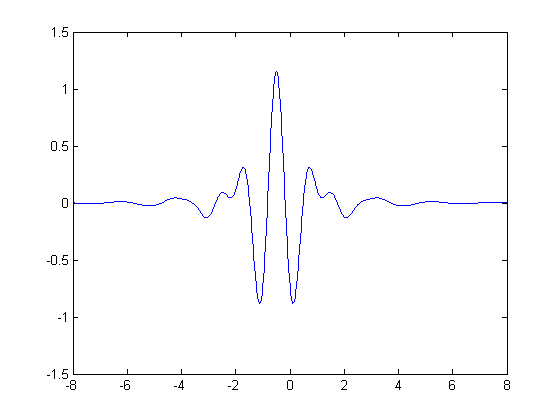
\includegraphics[width=3in]{Wavelet-Meyer}
  \caption{母小波示例}
  \label{fig:Wavelet-Meyer}
\end{figure}

\subsection{Wi-Fi信号简介}
\subsubsection{正交频分复用简介}
正交频分复用\upcite{nee2000ofdm}(Orthogonal Frequency Division Multiplexing,OFDM)是一种基于多载波,可以有效对抗频率选择性衰减,且具备高速率传输能力的传输技术。

解释OFDM前还要先介绍另外两个概念。调制,是指将欲传送的信号混合到载波中的过程,具体可以调制载波的相位、频率、幅度或者是三者的组合。子载波,是指将信道的可用频段进行为若干个子频段,工作在子频段上的载波即为子载波。

OFDM的基本思想是把要传输的数据分割为若干个子数据流,并将子数据流同时调制在多个彼此相互正交的子载波上传送。子载波带宽小,更接近于相关带宽,因此可以抵抗频率的选择性衰减。OFDM使用紧邻的子载波,每个子载波间不需要保护间隔,大大提高了带宽利用率。其中每个子载波采用传统的调制方式。因此OFDM是调制和复用的结合。

为避免子载波间相互干扰,OFDM对子载波间的正交性要求非常高。子载波的频率间隔需要满足公式~\ref{equ:ofdm}。
\begin{equation}
\label{equ:ofdm}
{x_m}\left( t \right) = \cos \left( {2\pi \left( {{f_c} + {f_m}} \right)t} \right) = {\mathop{\rm Re}\nolimits} \left( {{e^{j2\pi \left( {{f_c} + {f_m}} \right)t}}} \right) = {\mathop{\rm Re}\nolimits} \left( {{x_{lm}}\left( t \right){e^{j2\pi {f_c}t}}} \right)
\end{equation}

\subsubsection{Wi-Fi与802.11}

Wi-Fi指一种工作在无线局域网2.4GHz和5GHz频段下的无线局域网技术,其遵循802.11协议标准\upcite{zh2004ieee}。

802.11协议族是一系列基于同一基础标准的无线通信技术。无线局域网的第一个标准制定于1997年,即IEEE 802.11,随后又补充了802.11a,802.11b等一些列标准。其中与Wi-Fi有关的标准包括802.11a/b/g/n和802.11ac。协议族中详细定义了Wi-Fi的工作频段,信道划分等信息。例如在2.4G的频段下,Wi-Fi共有14个可用信道,图~\ref{fig:802channel}所示。
\begin{figure}[htbp] % use float package if you want it here
  \centering
  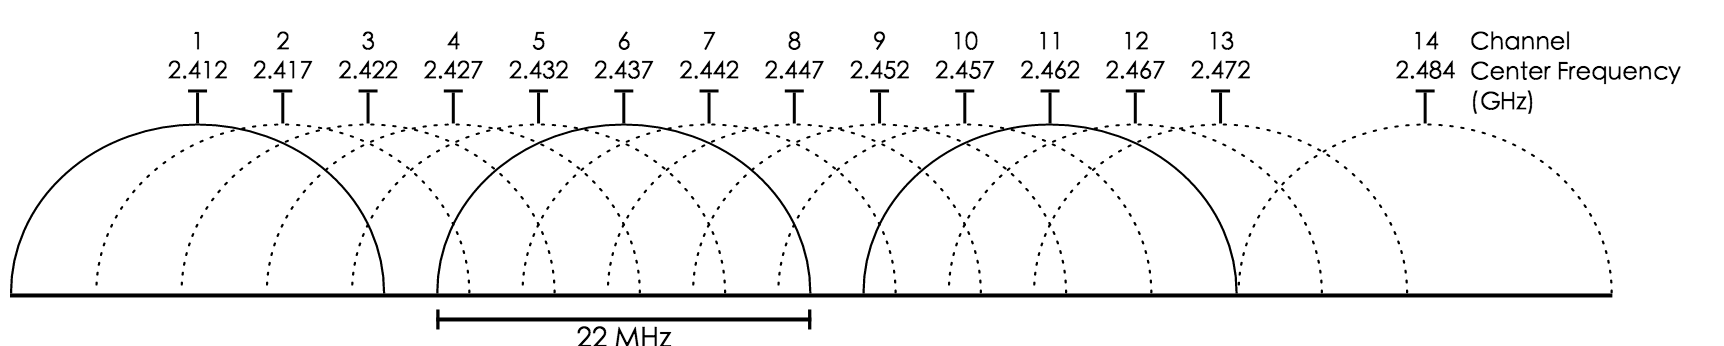
\includegraphics[width=5in]{802channel}
  \caption{2.4G下Wi-Fi的信道划分情况}
  \label{fig:802channel}
\end{figure}




















% \subsection{需求及要达到的目标}
% \subsubsection{用户是否在行走}
% \subsubsection{用户是否在使用手机}
% \section{现有的工作}

% \section{手机传感器工作原理}
% 正文内容
% \subsection{陀螺仪工作原理}
% 正文内容
% \subsection{加速传感器工作原理}
% 正文内容
% \subsection{距离传感器工作原理}
% 正文内容

% \section{系统设计}
% 正文内容
% 正文内容
% \subsection{手机传感器数据获取}

% \subsection{应用隐马尔可夫模型分析用户行走状态}
% 正文内容
% \subsection{数据融合与决策}

% \section{性能评估}
% 正文内容
% \subsection{实验设计}

% \subsection{结果与分析}

% \section{本章小结}

% 正文内容
% 引用示例:书的\upcite{tex, companion},
% 还有这些\upcite{Krasnogor2004e, clzs, zjsw},关于杂志的\upcite{ELIDRISSI94,
%   MELLINGER96, SHELL02},硕士论文\upcite{zhubajie, metamori2004},博士论文
% \upcite{shaheshang, FistSystem01},标准文件\upcite{IEEE-1363},会议论文\upcite{DPMG,kocher99},%
% 技术报告\upcite{NPB2}。中文参考文献\upcite{cnarticle}\textsf{特别注意}





